\documentclass{article}
\usepackage{amsmath}
\usepackage{mathtools}
\usepackage{gensymb}
\usepackage[a4paper,inner=1.5cm,outer=1.5cm,top=2cm,bottom=0.5cm]{geometry} 
\usepackage{xcolor}                    
\usepackage{tikz}                           
\usepackage{multicol}
\usepackage{pgfplots}
\usetikzlibrary{calc}
\usetikzlibrary{intersections}
\usetikzlibrary{intersections,calc,angles,quotes}
\usetikzlibrary{shapes,arrows,positioning,decorations.pathreplacing,calc}
\usetikzlibrary{calc,angles,positioning,intersections,quotes,decorations.markings}
\usepackage{tkz-euclide}
\usetikzlibrary{backgrounds}
\usetikzlibrary{calc,through}
\usetikzlibrary{angles}
\usetikzlibrary{fadings}
\usetikzlibrary{shapes.geometric}
\usetikzlibrary{shapes.symbols}
\usepackage{draftwatermark}
\usepackage{mathptmx}

\SetWatermarkText{\textcolor{black!30}{Mathema Shukur}}
\SetWatermarkFontSize{2 cm}
\usepackage[utf8]{inputenc}
\usepackage{fontspec}

\setmainfont{[Kalpurush.ttf]}
\newfontface{\en}{[Arial.ttf]} %%this is optional, if you want to use a secondary font. Any english font is supported
\newlength\Radius
\setlength\Radius{4cm}
\begin{document} 
	\Large
	\textcolor{red}{Welcome To} 
	\\
	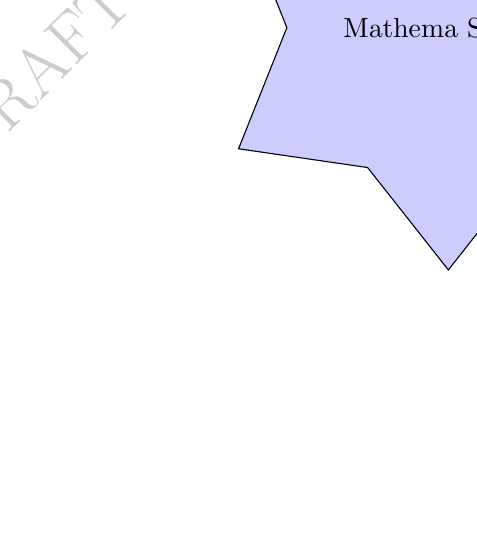
\begin{tikzpicture}
		\tikz \node [fill=blue!20,star,star points=6,draw] {Mathema Shukur };
	\end{tikzpicture}
	\\
	যাদের জন্যে প্রযোজ্যঃ  	\textcolor{magenta}{একাদশ ও দ্বাদশ শ্রেণীর শিক্ষার্থী} \\
	বিষয়ঃ \textcolor{magenta}{উচ্চতর গণিত ১ম পত্র} \\
	অধ্যায়ঃ \textcolor{magenta}{৩-সরলরেখা}\\ 
	Subtopicঃ  \textcolor{magenta}{চলমান বিন্দুর সঞ্চার পথের সমীকরণ নির্ণয় locus of a moving point }\\
	\\
	নির্দিষ্ট শর্তাধীনে চলমান বিন্দু সমূহের সেটকে সঞ্চার পথ (Locus) বলে। \\
	\\
	$t$	এর সকল বাস্তব মানের জন্য একটি বিন্দুর স্থানাঙ্ক $(at^2,2at)$ হলে বিন্দুটির সঞ্চার পথের সমীকরণ নির্ণয় কর \\
	\\ 
	$(x,y)=(at^2,2at)$\\
	\begin{multicols}{2}
		\begin{align*}
			y&=2at\\
			\\
			t&=\frac{y}{2a}
		\end{align*}
		\\
		\begin{align*}
			x&=a\,\,t^2\\
			\\
			x&=a\,\,\left(\frac{y}{2a}\right)^2\\
			\\
			x&=\frac{y^2}{4a}\\
			\\
			y^2&=4\,a\,\,x
		\end{align*}
	\end{multicols}
\begin{tikzpicture}
	\draw[->] (-1, 0) -- (8, 0) node[right] {$x$};
	\draw[->] (0, -5) -- (0, 4.2) node[above] {$y$};
	\draw[scale=1, domain=-3:3, smooth, variable=\y, red,dashed]  plot ({\y*\y}, {\y});
		\node at (3,1) {$\textcolor{blue}{(at^2,2at)}$};	
			\node at (6,2) {$\textcolor{blue}{	y^2=4\,a\,\,x}$};
			\fill[red] (2,1.4) circle (0.5 mm);
\end{tikzpicture}
\\
	কোনো সেটের একটি বিন্দু এমন যে, মূলবিন্দু হতে বিন্দুটির দূরত্ব $y-$ অক্ষ রেখা থেকে  তার দূরত্বের দ্বিগুন, বিন্দুটির সঞ্চার পথের সমীকরণ নির্ণয় কর\\
	\\
	মনে করি, সেটের একটি বিন্দু $P(x,y)$ \\
	\\
	মূলবিন্দু $O(0,0)$  হতে $P(x,y)$ বিন্দুটির দূরত্ব\\
	\\ 
	$OP=\sqrt{(x-0)^2+(y-0)^2}=\sqrt{x^2+y^2}$\\
	\\ 
	$y-$ অক্ষ রেখা থেকে $P(x,y)$ বিন্দুটির দূরত্ব $=|x|$\\
	\\ 
	\begin{align*}
		\sqrt{x^2+y^2}&=2|x|\\
		\\
		x^2+y^2&=4\,\,x^2\\
		\\
		y^2&=3\,\,x^2
	\end{align*}
\\
	কুমিল্লা বোর্ড-২০২১\\ 
$(2,-1)$ বিন্দু থেকে যে সেটের বিন্দু সমূহের দূরত্ব  $4$ একক সেই সঞ্চারপথ নির্ণয় কর\\ 
\\
মনে করি, সেটের একটি বিন্দু $P(x,y)$ \\
\\
সুতরাং $P(x,y)$  বিন্দু থেকে $A(2,-1)$ বিন্দুর দূরত্ব  $4$ \\
\\
$\boxed{\textcolor{blue}{d=\sqrt{(x_1-x_2)^2+(y_1-y_2)^2}}}$\\
\\ 
$PA=\sqrt{(x-2)^2+(y+1)^2}$\\
\\
$PA=4$\\
\\
$\sqrt{(x-2)^2+(y+1)^2}=4$\\
\\
$(x-2)^2+(y+1)^2=16$\\ 
\\
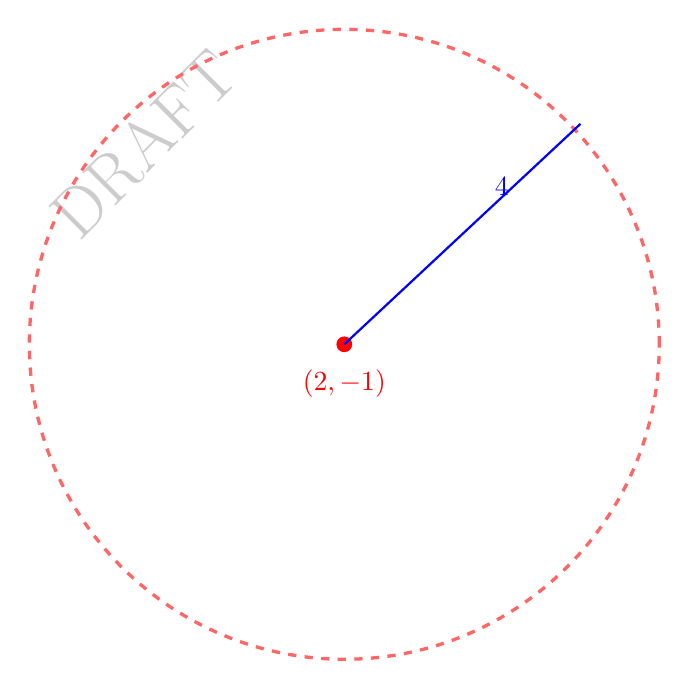
\begin{tikzpicture}
	\draw[color=red!60, very thick,dashed](2,-1) circle (4);
		\fill[red] (2,-1) circle (1 mm);
			\node at (2,-1.5) {$\textcolor{red}{(2,-1)}$};	
		\draw[thick,blue] (2,-1)--(5,1.8);	
			\node at (4,1) {$\textcolor{blue}{4}$};	
\end{tikzpicture}
\\
দিনাজপুর বোর্ড-২০১৫\\ 
$A(2,3)$ এবং  $B(-1,4)$ দুইটি স্থির বিন্দু । একটি সেট এমনভাবে গঠন করা হয়েছে যে  $A$ ও  $B$ বিন্দু থেকে সেটের যেকোনো একটি বিন্দুর দূরত্বের অনুপাত সর্বদা $2:3$;  সঞ্চার পথের সমীকরণ নির্ণয় কর  \\
\\
মনে করি, সেটের একটি বিন্দু $P(x,y)$ \\
\\
সুতরাং  $A(2,3)$  ও  $B(-1,4)$  বিন্দু থেকে সেটের  $P(x,y)$ বিন্দুর দূরত্বের অনুপাত সর্বদা $2:3$; \\
\\
$\boxed{\textcolor{blue}{d=\sqrt{(x_1-x_2)^2+(y_1-y_2)^2}}}$\\
\\ 
$PA=\sqrt{(x-2)^2+(y-3)^2}$\\
\\
$PB=\sqrt{(x+1)^2+(y-4)^2}$\\
\\
\begin{align*}
	PA: PB&=2:3\\
	\\
	\frac{PA}{PB}&=\frac{2}{3}\\
	\\
	\frac{\sqrt{(x-2)^2+(y-3)^2}}{\sqrt{(x+1)^2+(y-4)^2}}&=\frac{2}{3}\\
	\\
	\frac{(x-2)^2+(y-3)^2}{(x+1)^2+(y-4)^2}&=\frac{4}{9}\\
	\\
	9(x-2)^2+9(y-3)^2&=4(x+1)^2+4(y-4)^2\\
	\\
	9(x^2-4x+4)+9(y^2-6y+9)&=4(x^2+2x+1)+4(y^2-8y+16)\\
	\\
		9x^2-36x+36+9y^2-54y+81&=4x^2+8x+4+4y^2-32y+64\\
		\\
		5x^2+5y^2-44x-22y+49&=0
\end{align*}
	\begin{tikzpicture}[transform shape,scale=1]
	\draw [-latex,thick](-6,0) -- (6,0) node[right] {$x$} coordinate(x axis);
	\draw [-latex,thick](0,-6) -- (0,6) node[above] {$y$} coordinate(y axis);
	\fill[black] (0,0) circle (0.5 mm);
	\node at (0.3,-0.3) {$\textcolor{purple}{O}$};	
	\draw[thick,magenta] (5,5)--(-5,-5);
	\node at (1.5,0.4) {$\textcolor{blue}{45\degree}$};	
	\node at (4,2) {$\textcolor{blue}{m=\tan \theta }$};	
	\node at (4,1) {$\textcolor{blue}{m=\tan 45\degree=1 }$};
	\node at (5,5.5) {$\textcolor{magenta}{A}$};
	\node at (-5,-5.5) {$\textcolor{magenta}{B}$};			
	\draw[color=blue,ultra thick, ->] (1,0) arc (0:45:1cm);
\end{tikzpicture}
\end{document}